\documentclass{article}
\usepackage{tikz}

\begin{document}

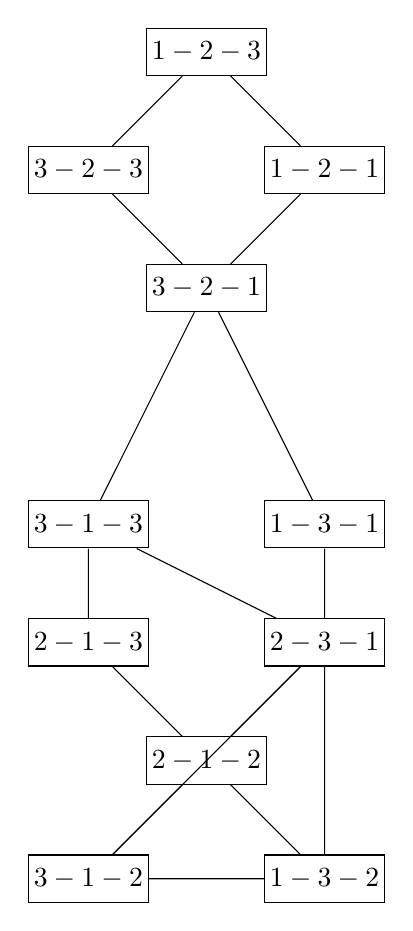
\begin{tikzpicture}[scale=1.5]
    % Define node styles
    \tikzstyle{vertex}=[draw, rectangle, minimum size=6mm, inner sep=2pt]
    
    % Draw nodes
    \node[vertex] (a) at (0,0) {\(1-2-3\)};
    \node[vertex] (b) at (-1,-1) {\(3-2-3\)};
    \node[vertex] (c) at (1,-1) {\(1-2-1\)};
    \node[vertex] (d) at (0,-2) {\(3-2-1\)};
    \node[vertex] (e) at (-1,-4) {\(3-1-3\)};
    \node[vertex] (f) at (1,-4) {\(1-3-1\)};
    \node[vertex] (g) at (-1,-5) {\(2-1-3\)};
    \node[vertex] (h) at (1,-5) {\(2-3-1\)};
    \node[vertex] (i) at (0,-6) {\(2-1-2\)};
    \node[vertex] (j) at (-1,-7) {\(3-1-2\)};
    \node[vertex] (k) at (1,-7) {\(1-3-2\)};
    
    % Draw edges
    \draw (a) -- (b);
    \draw (a) -- (c);
    \draw (b) -- (d);
    \draw (c) -- (d);
    \draw (d) -- (e);
    \draw (d) -- (f);
    \draw (e) -- (g);
    \draw (e) -- (h);
    \draw (f) -- (h);
    \draw (g) -- (i);
    \draw (h) -- (i);
    \draw (h) -- (j);
    \draw (h) -- (k);
    \draw (i) -- (j);
    \draw (i) -- (k);
    \draw (j) -- (k);
\end{tikzpicture}

\end{document}